\section{Anforderungsanalyse}

% Merkmale Cloud Native Anwendungen
% Was muss Applikation hierzu erfüllen (non-functional requirements)?

Um ein Migrationskonzept entwerfen zu können wird zuerst die existierenden Anwendung kurz beschrieben und untersucht und mithilfe einer Literaturrecherche die notwendigen Anforderungen an die Migration erarbeitet.

\subsection{Existierender Code}
Ziel der Anwendung ist das Einsammeln der Timesheets, in dem Projekt aktiver Mitarbeiter, aus einem \gls{Box} Verzeichnis, das Überprüfen dieser und die anschließende Rechnungs- und Report Erstellung. Die Prozesse werden jeweils manuell über eine Konsoleneingabe gestartet. Im \gls{Box}-Verzeichnis liegt ein Projektmanagement-File, welcher alle Mitarbeiter enthält, die jemals in dem Projekt gearbeitet haben und markiert, welche auch aktuell aktiv sind und dem Kunden in Rechnung gestellt werden können. Außerdem sind in dem Verzeichnis auch die Reports aus einem Zeiterfassungstool abgelegt. In Abbildung \ref{fig:pmo_python} wird der Aufbau der ursprünglichen Anwendung dargestellt.

\begin{figure}[H]
    \centering
    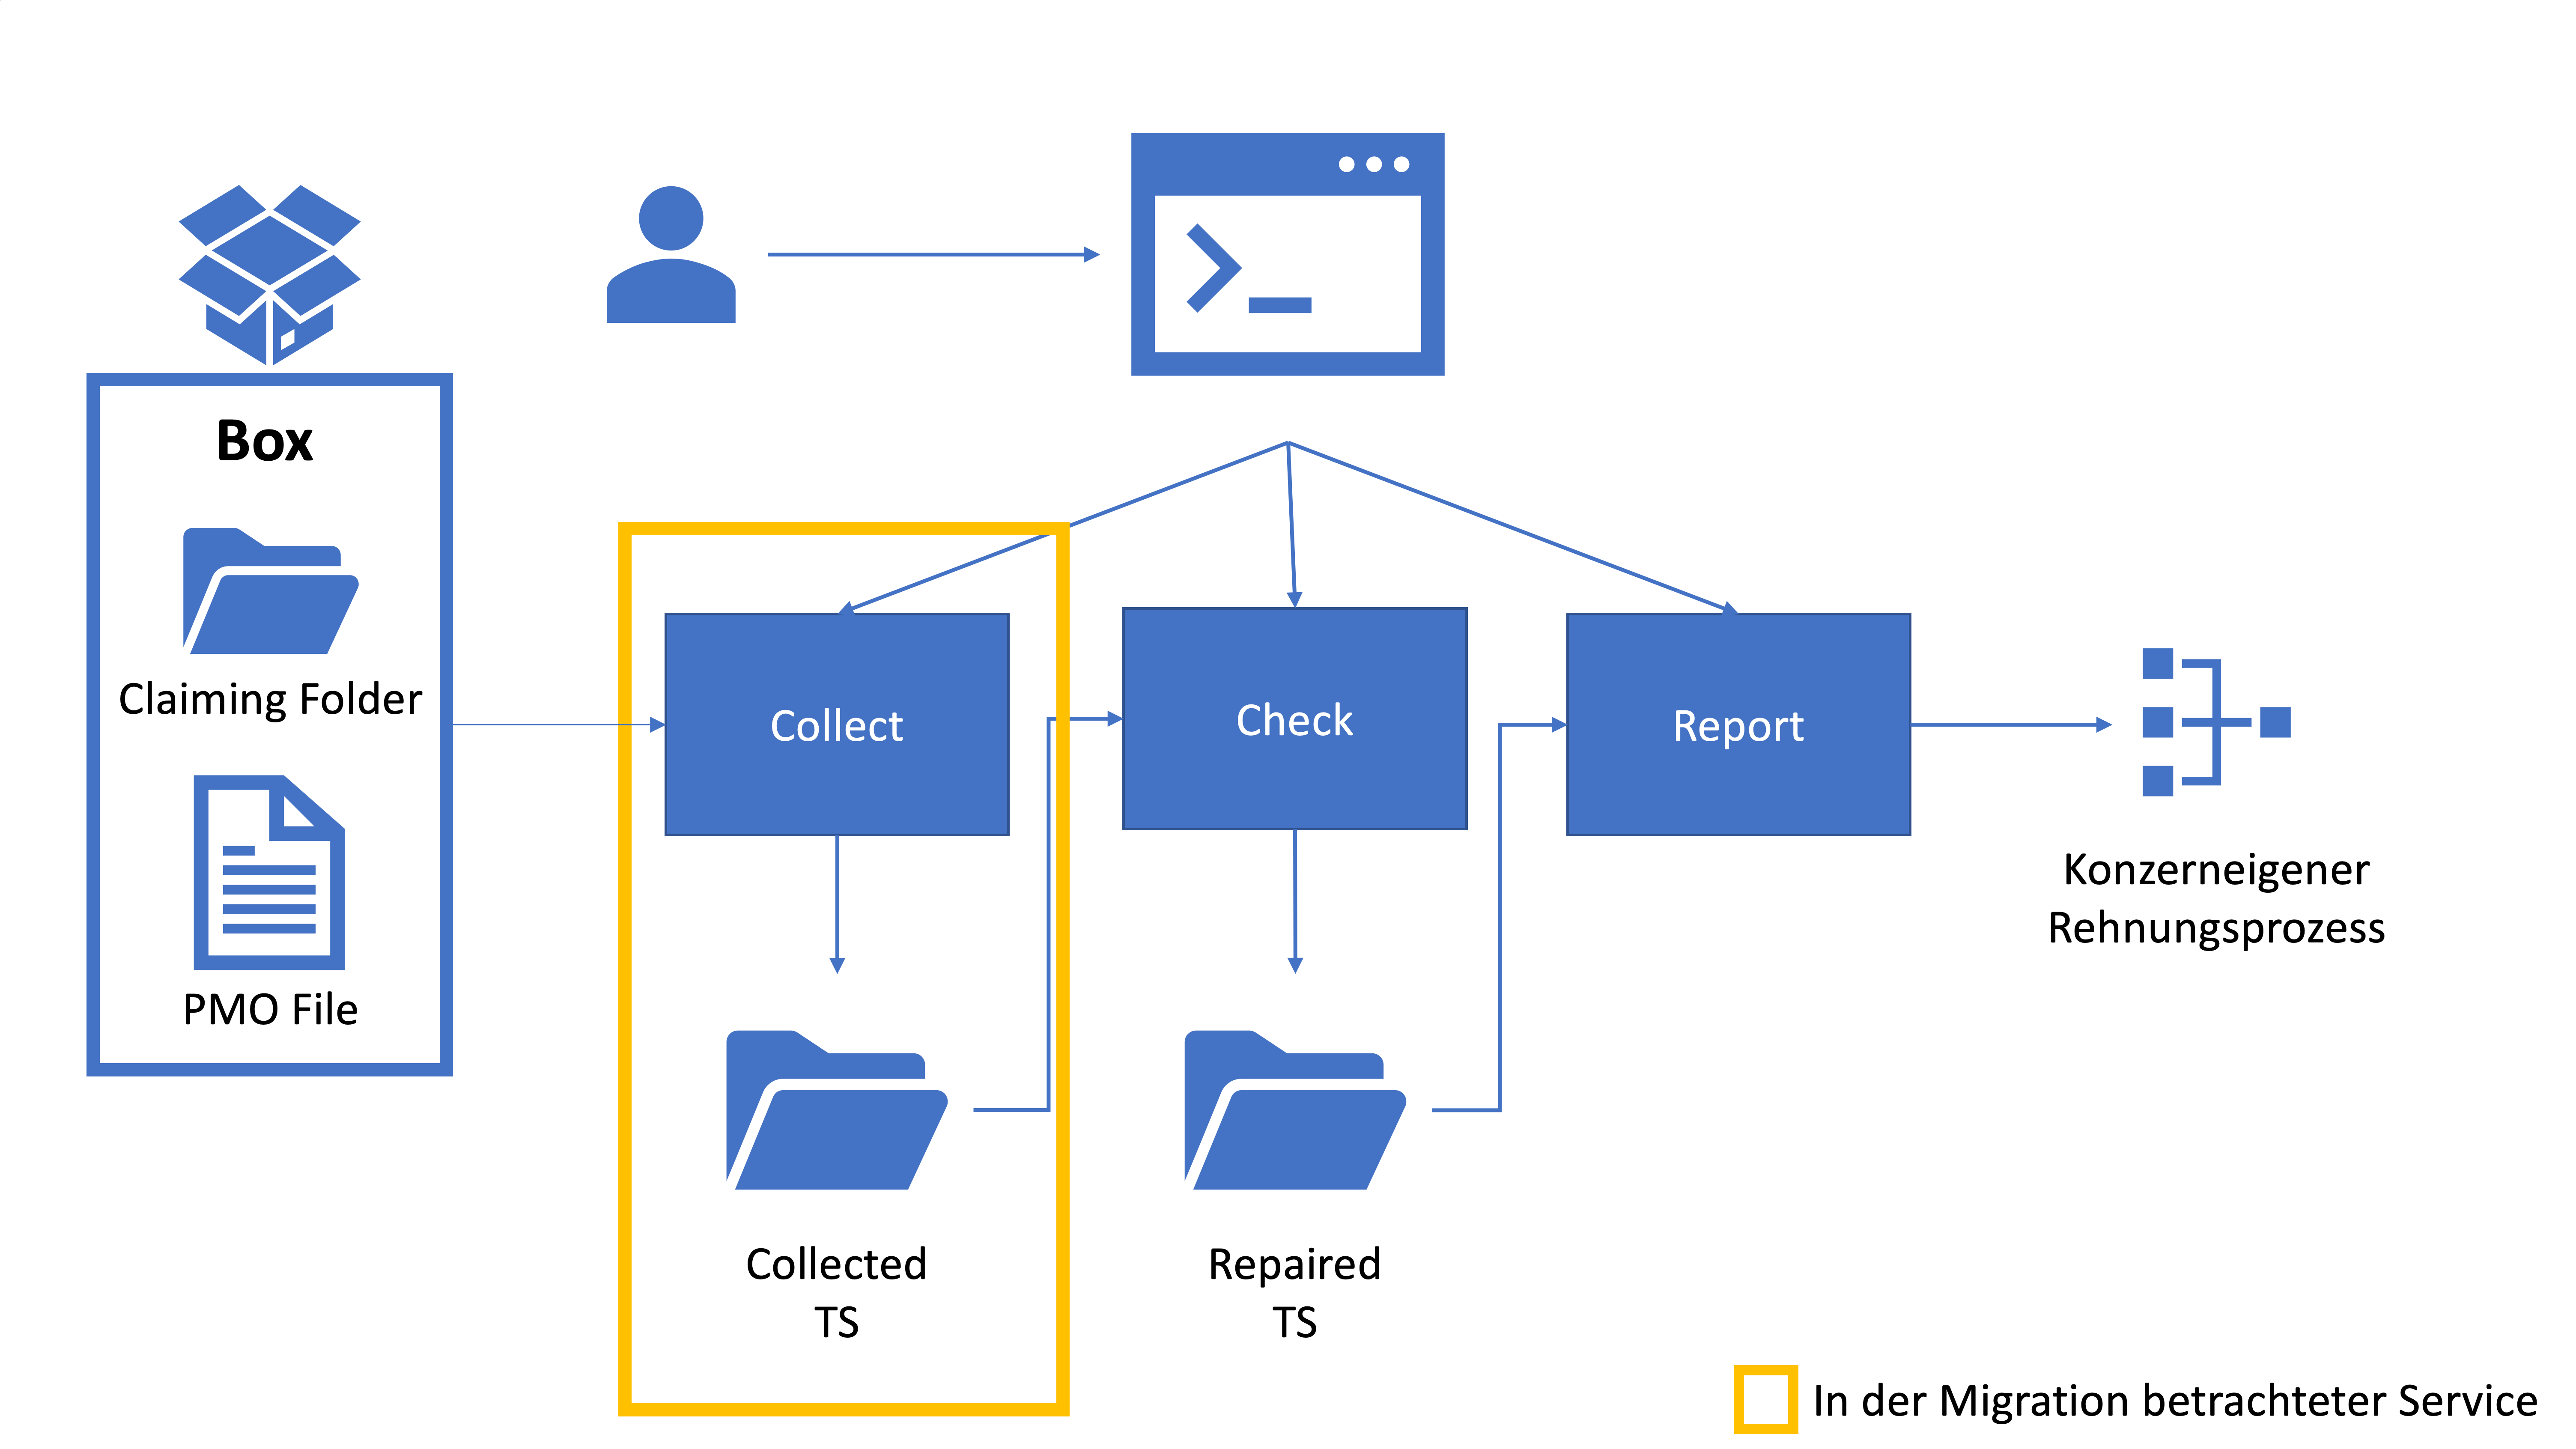
\includegraphics[width=0.65\textwidth]{pmo_python.png}
    \caption{Aufbau der ursprünglichen Anwendung (gelb umrandet der Teil, der prototypisch migriert wird)}
    \label{fig:pmo_python}
\end{figure}

Die bisher existierende Anwendung ist eine Python Anwendung, die grundsätzlich in dre Module aufgeteilt ist:
\begin{itemize}
\item \textbf{Timesheet Collector: }Einsammeln der Timesheets, der in dem Projekt aktiven Mitarbeiter
\item \textbf{Timesheet Checker: }Überprüfen der Timesheets auf Korrektheit und Vollständigkeit und gegebenenfalls Reparatur dieser
\item \textbf{Report Creator: }Erzeugung eines Reports, Zusammenfassung der \textit{reporteten} Stunden und Verteilung dieser auf die unterschiedlichen Beauftragungen, Erstellung von Nachweisdokumenten und automatisierte Rechnungsstellung
\end{itemize}

Jeder dieser drei Services ist ein eigenes Python Modul. Diese greifen jeweils auf weitere Services wie einen Excel-Helper und Checking-Tools zurück.

Da es sich bei dieser Arbeit um eine Machbarkeitsstudie mit Erstellung eines Prototypen handelt, wird im ersten Schritt nur die Migration des Collect Service untersucht, bevor die anderen, komplexeren Services migriert werden. Dies ist in Abbildung \ref{fig:pmo_python} entsprechend durch den gelben Rahmen gekennzeichnet. Der Collect Service benötigt eine Verbindung zu dem \gls{Box}-Verzeichnis und einen Ablageort für die \glqq{eingesammelten}\grqq{} Timesheets.

\subsection{Anforderungen an die Cloud Migration}
Wird eine Anwendung in die Cloud migriert werden unter anderem folgende Vorteile erwartet \cite[Vgl. auch im Folgenden][03:23-05:36min]{AWS2019}:
\begin{itemize}
\item Kostensenkung
\item Steigerung der Produktivität
\item Agilität in der Entwicklung
\end{itemize}

Darüber hinaus muss vor der Migration untersucht und festgelegt werden, welche der in Kapitel \ref{sec:migrationsansaetze} herausgearbeiteten Migrationsstrategien verfolgt werden soll \cite[Vgl.][10:38-13:23min]{AWS2019}. Jede dieser Strategien bietet ihre Vor- und Nachteile, weshalb diese Entscheidung individuell von der Anwendungsarchitektur und der Art der Benutzung abhängig ist. \pagebreak

Grundlegend kann der Migrationsprozess  in vier Schritte zusammengefasst werden \cite[Vgl. auch im Folgenden][S. 34f]{Maenhaut2016}:
\begin{enumerate}
\item \textbf{Auswahl der Komponenten:} Die Auswahl der zu migrierenden Komponenten sollte als erster Schritt vorgenommen werden. Wird die ganze Anwendung migriert ist dieser entsprechend einfach. Zu beachten ist hier vorallem die Kommunikation zwischen den Komponenten und damit verbundenen Sicherheitsanforderungen.
\item \textbf{Feststellen kompatibler Cloud Provider:} Verschiedene Provider bieten verschiedene Möglichkeiten und haben unterschiedliche limitierende Faktoren. Somit sollte ein Provider gefunden werden, der alle gewünschten Features abdecken kann.
\item \textbf{Einfluss auf das Client Netzwerk untersuchen:} Da die Kommunikation zwischen einzelnen Komponenten ins Internet verlagert wird, muss möglicher Weise die Bandbreite des Client Netzwerks angehoben werden.
\item \textbf{Skalierung der Anwendung:} Einer der Vorteile des Cloud Computing ist die Skalierbarkeit, also die Fähigkeit, bei großer Last weitere Instanzen einer Anwendung zu starten. Um diese Skalierbarkeit bereitstellen zu können müssen die Komponenten lokalisiert werden, die entsprechend angepasst werden müssten.
\end{enumerate}

% Thema Sicherheit ?!

Bei dem in dieser Arbeit untersuchten Prototypen werden alle Komponenten des Collect Service migriert, weshalb keine speziellen Komponenten ausgewählt werden müssen oder die Kommunikation zwischen diesen geprüft werden muss. Somit ist der erste Schritt recht einfach abzuschließen. Die Auswahl eines Passenden Providers wird im weiteren Verlauf dieser Arbeit beschrieben. Einen Einfluss auf das Client Netzwerk wird der Prototyp nicht haben, es sollte lediglich hinsichtlich der Auswahl des Cloud Providers darauf geachtet werden, dass die Netzwerkanbindung ausreicht um zum Beispiel das Projektmanagement-File zuverlässig herunterzuladen. Die Skalierbarkeit der Anwendung bleibt für den ersten Prototypen vorerst außerhalb der Zielsetzung, diese würde erst nach einer erfolgreichen Machbarkeitsstudie weiter betrachtet werden.

Zudem ist zu untersuchen, ob eine Public, Hybrid oder Private Cloud verwendet werden kann. Für den Prototypen ist der Einsatz einer Public Cloud Infrastruktur unproblematisch, da hier nur Testdatensätze verwendet werden. Würden die realen Daten verwendet, so müsste auf eine Private Cloud umgestellt werden, da die Timesheets personenbezogene Daten enthalten und unternehmenskritische Daten wie Informationen über das Budget und Gewinn/Verlust im PMO-File enthalten sind.

Darüber hinaus soll eine Anwendung in der Cloud je nach Bedarf auch von mehr Nutzern gleichzeitig nutzbar sein, weshalb auch über die Umsetzung von \textit{multi-tenancy} nachgedacht werden sollte \cite[Vgl.][S. 34ff]{Maenhaut2016}. Im Falle des in dieser Arbeit beschriebenen Prototypen ist das jedoch erst einmal nicht nötig.
\pagebreak